\section{Introduction}

The practice of investors jointly funding the same venture is known as  syndication. It plays a central role in innovation financing by allowing investors to pool expertise, share risk and signal project quality to the market \cite{Lerner1994,Casamatta2007}.  

Despite its practical importance, most empirical studies analyse syndication at the firm or deal level and provide limited insight into the system‑level patterns through which investors coordinate \cite{Pruthi2005, Benzouai2021}.  Understanding how these patterns emerge requires a multidisciplinary perspective encompassing finance, sociology, Network Science and ecology.

This collaborative behavior also reflects information asymmetries and screening challenges inherent in investment markets \cite{Lerner1994}, as in incomplete information environments, investors rely on social relationships to reduce uncertainty and improve screening efficiency.

In venture capital markets (innovation financing included), syndication serves as a coordination mechanisms used by Venture Capitalists (VCs) to operate in complex networks where investment decisions are embedded within social structures, geographic clusters, and institutional relationships. 

% However, traditional approaches to studying venture capital often focus on individual investment decisions or firm-level characteristics \cite{Pruthi2005, Benzouai2021}, leaving the broader systemic patterns of investor coordination (e.g. syndication) to be further explored.

This study aims to apply Network Science theories and methods to analyze these coordination patterns in the syndication network of early and late stage investors operating in the U.S. market, revealing how investors organize into distinct network communities with different structural properties and organizational patterns that may influence capital allocation efficiency, deal flow, and market access.

Special attention is given for the fact that a community of proiminent VCs in the Sylicon Valley  demonstrate nested hierarchical organization patterns, while others maintain more random, hard-to-define partnership structures.

The following sections examine the theoretical foundations for syndication behavior, drawing from literature in innovation financing, social embeddedness, network theory, and ecological systems to build a comprehensive framework for understanding syndication investments networks organization. 

Nevertheless, implications on market efficiency, geographic clustering effects, and the role of innovation hubs in shaping investment ecosystems is discussed, as well as future reasearch opportunities are presented.

\subsection{Syndication in Innovation Financing}

Theoretical foundations for syndication behavior comes from literature on screening and information sharing among venture capitalists \cite{Casamatta2007}. Syndication became relevant in that context because, in markets characterized by incomplete information (e.g. innovation financing), the decision to syndicate and the choice of syndication partners are aspects that influence both investment outcomes and network position \cite{Casamatta2007}.

In innovation financing, when investors face uncertainty about startup quality and potential, syndication serves multiple strategic functions: it enables knowledge pooling from partners with complementary expertise \cite{Lerner1994}, reduces individual exposure to high-risk ventures, and provides valuable signals \cite{Spence1981} about investment quality through the revealed preferences of co-investors. 

In this context, considering that screening innovative ventures is frequently a multi-stage process (venture capitalists define formal pipeline which startups and often their founders need to pass through), syndication plays an important role to reduce the effort and possibilty the number of screening stages, with the cost of disclousring information, as investors are essencially competitors.

\subsection{Economic Sociology and Embeddedness}

Economic sociologists have shown that economic action is embedded in ongoing social networks \cite{Granovetter1985}; entrepreneurs and venture capitalists form recurring partnerships based on trust and reputation \cite{Uzzi1997}.  The concept of structural holes \cite{Burt1992} highlights that brokers who bridge otherwise disconnected groups can access unique information and control resource flows.  Geographic clustering in innovation hubs, such as Silicon Valley, facilitates repeated interactions and strengthens these social ties, potentially shaping syndication patterns.

In venture capital markets, embeddedness manifests in several important ways. First, investment decisions are embedded within social networks where venture capitalists develop recurring partnerships based on trust, shared investment philosophies, and successful collaboration histories \cite{Granovetter1985}. These relationships create persistent patterns of co-investment that go beyond individual deal characteristics, forming the basis for community structure within investor networks.

Second, geographic embeddedness plays a critical role in shaping investor relationships. Venture capitalists concentrated in innovation hubs like Silicon Valley develop dense local networks through frequent face-to-face interactions, shared professional communities, and common institutional affiliations \cite{Granovetter1985}. This geographic clustering creates information advantages and relationship-building opportunities that can influence syndication patterns and network organization.

Third, embeddedness creates informal hierarchies of influence and reputation within investor communities. Rather than operating as independent agents, investors form interconnected networks that share information, coordinate investment strategies, and establish social rankings based on past performance and network position \cite{Granovetter1985}. These social hierarchies can evolve into the structural hierarchies measured through nestedness analysis.

The embeddedness perspective helps explain why certain investor communities develop systematic organizational patterns while others remain more randomly structured. Social relationships, trust networks, and geographic proximity may facilitate the emergence of hierarchical organization by creating conditions where, for instance, specialists naturally align with generalists' investment strategies (not purely random). This social foundation provides the context for understanding how network topology emerges from underlying social processes rather than purely market-driven mechanisms.

\subsection{Network Science and Syndication Networks}

In this work, we use Network Science as an umbrella term that brings together (i) network theory (how positions and ties affect outcomes), (ii) the theory of networks (how structures arise), and (iii) the graph-theoretic foundations and metrics that make these analyses possible.

Network theory (i) looks at how mechanisms and processes operating through a given network produce outcomes for people and groups. Using \cite{VargasHernandez2019}’s distinction, it focuses on, for instance, what happens when someone has many connections, sits in a central position, or bridges others. The core question is: given a structure, what consequences follow for actors and collectives? 

By contrast, theory of networks (ii) asks about the causes of structure—the antecedents of network properties in Brass’s terms. It models who connects to whom, what kinds of ties they form, who becomes central, and which whole-network patterns appear (such as high centralization or small-world path lengths). The core question here is: what processes make the network take the shape it has?

Under both views sits graph theory (iii), the math of networks. It gives precise definitions of nodes and edges, paths and distances, and the core measures we use (degree, centrality, clustering, connectivity). These tools let us describe a network’s shape, test ideas about causes and effects, and compare cases. Network Science (as a broader field) builds on this math to study system-level patterns, and statistics helps with modeling and uncertainty.

In the following sub-sections we explore concepts spaning all of those fields to set the theorical basis to our reasoning on the syndication networks analysis for furhter chapters.

\subsubsection{Unipartite and Bipartite Networks}

Understanding the distinction between unipartite and bipartite network representations is fundamental to our analysis of investor syndication patterns, as it determines our ability to identify hierarchical structures like nestedness that emerge from role differentiation between network participants.

A unipartite network has a single set of nodes, and any two nodes may be linked (e.g., people connected to people). A bipartite network has two disjoint sets of nodes that play different roles, and links are allowed only between the sets (e.g., plants–pollinators \cite{Dormann2009} or early–late investors), never within a set. Bipartite models are useful when role separation matters; unipartite views can be obtained by projecting a bipartite network onto one side. 

These network types differ fundamentally in their matrix representations: unipartite networks are represented by square matrices where all nodes appear in both rows and columns (known as adjacency matrix), while bipartite networks use rectangular matrices where rows represent one node group and columns represent the other (biadjacency matrix), as illustrated in Figure~\ref{fig:unipartite_vs_bipartite}. 

This matrix structure is crucial because nestedness patterns—characterized by the triangular arrangement of non-zero entries when ordered by degree—can only be properly identified in the rectangular bipartite matrix format. Moreover, ecological concepts like nestedness (which we will employ to analyze investor hierarchies) are most naturally defined and measured in biadjacency matrices.

\begin{figure}[htbp]
    \centering
    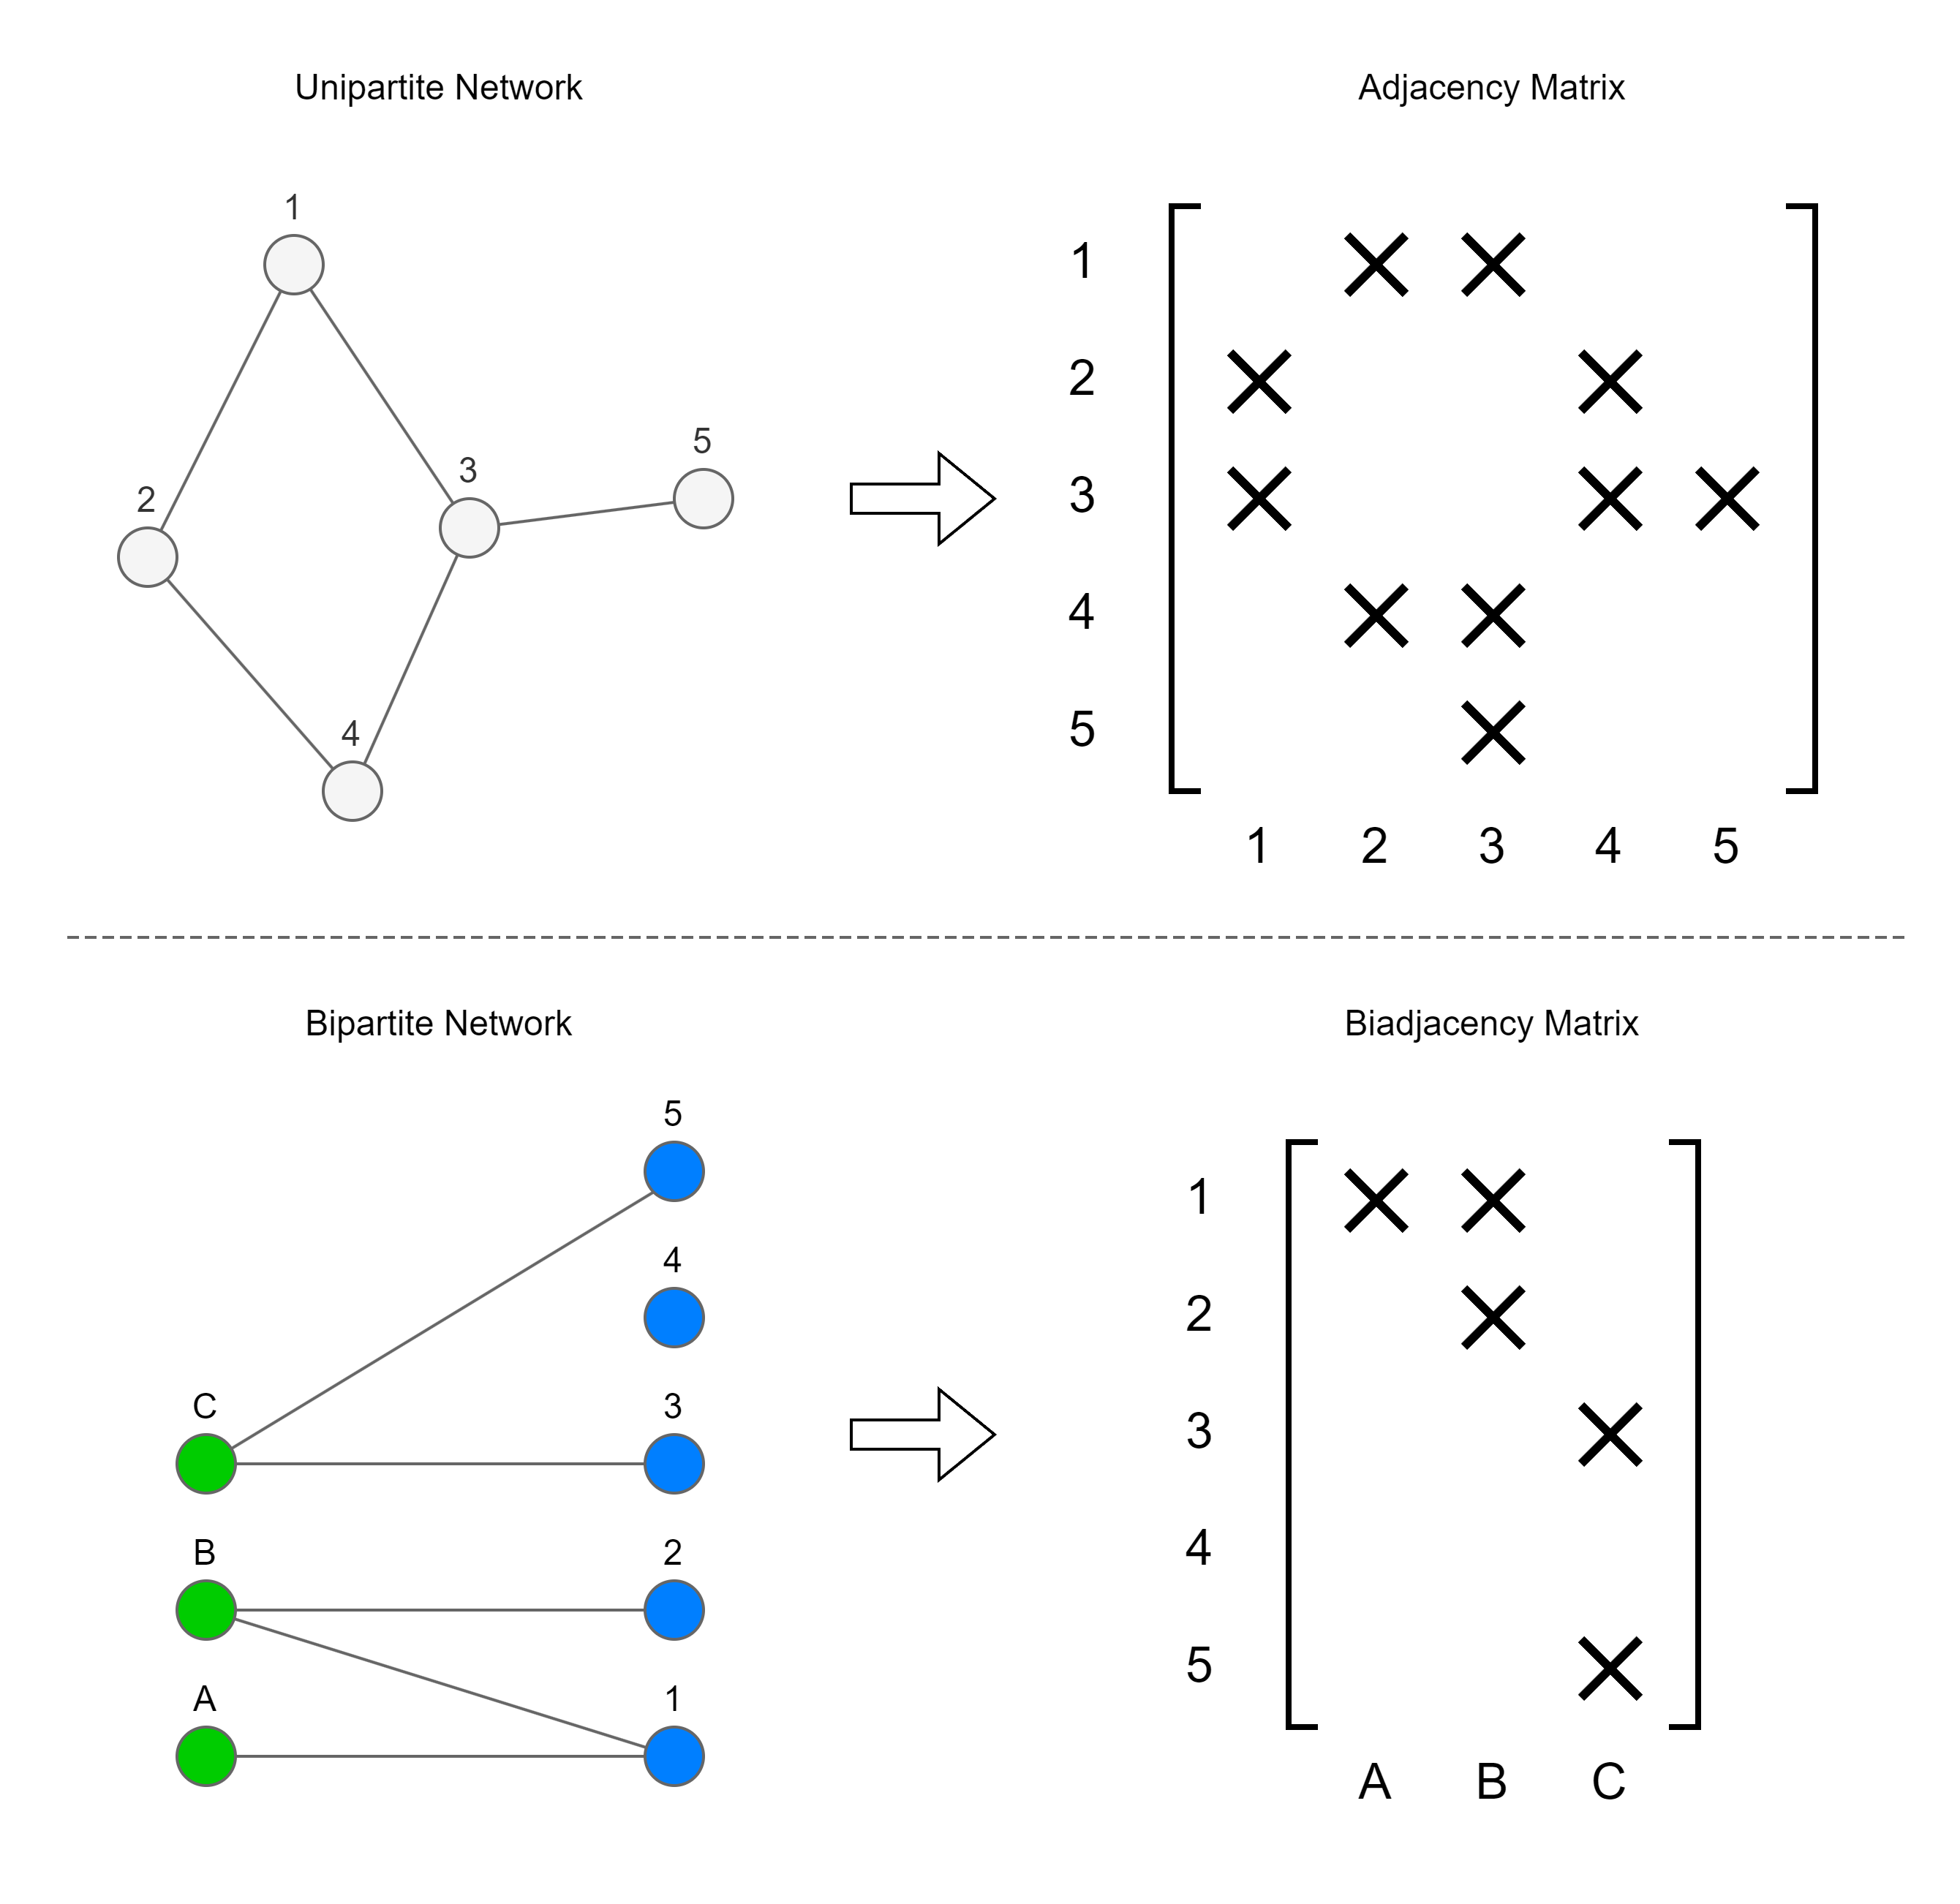
\includegraphics[width=0.8\textwidth]{../diagrams/unipartite_vs_bipartite_networks.png}
    \caption{Top, a unipartite network—one set of nodes (white) where edges can connect any pair. Bottom, a bipartite network—two disjoint sets (green vs. blue) with edges only across sets and none within a set. Respective adjacency and biadjacency matrix on right side, where "X" is actually substituted by "1" for calculations.}
    \label{fig:unipartite_vs_bipartite}
\end{figure}

In our context, modeling investors and companies as distinct node sets in a bipartite framework allows us to capture the role-specific interactions that generate nested patterns, whereas traditional unipartite investor-investor projections \cite{Bygrave1987} would obscure these hierarchical relationships. 

As we will demonstrate in the methodology section and through ecological analogies, the bipartite representation preserves the structural information necessary to transpose interpretations from mutualistic ecological systems to economic and social systems. The figure below contrasts these two cases.

\subsubsection{The Classical Syndication Model}

In co‑investment networks, investors are nodes and shared funding rounds are edges. Network measures quantify centrality, detect community structure and reveal degree heterogeneity \cite{Borgatti2009,Newman2003}. Many real‑world networks, including VC ecosystems, exhibit heavy‑tailed degree distributions generated by preferential attachment dynamics \cite{Barabasi1999}, and so they display small‑world characteristics, combining local clustering with short global path lengths \cite{Watts1998}. 

The classical approach to studying venture capital syndication treats all investors as a single group and connects them whenever they participate in the same funding round \cite{Bygrave1987}. In this model, investors are represented as nodes in a network, and an edge is drawn between any two investors who have co-invested in at least one company together.

This traditional view creates a unipartite network where, for instance, if Investor 1, Investor 2, and Investor 3 all participate in funding Company E, then it creates direct connections between 1-2, 1-3, and 2-3, as illustrated in Figure~\ref{fig:classical_syndication_net}. The resulting network shows the web of relationships among all investors based on their shared investment activities.

While this approach has been widely used in venture capital research \cite{Bygrave1987}, it treats all investors identically regardless of their roles in the investment process. Early-stage investors who specialize in seed funding are connected in the same way as late-stage investors who focus on growth capital, even though their investment strategies and market positions may be fundamentally different.

\begin{figure}[htbp]
    \centering
    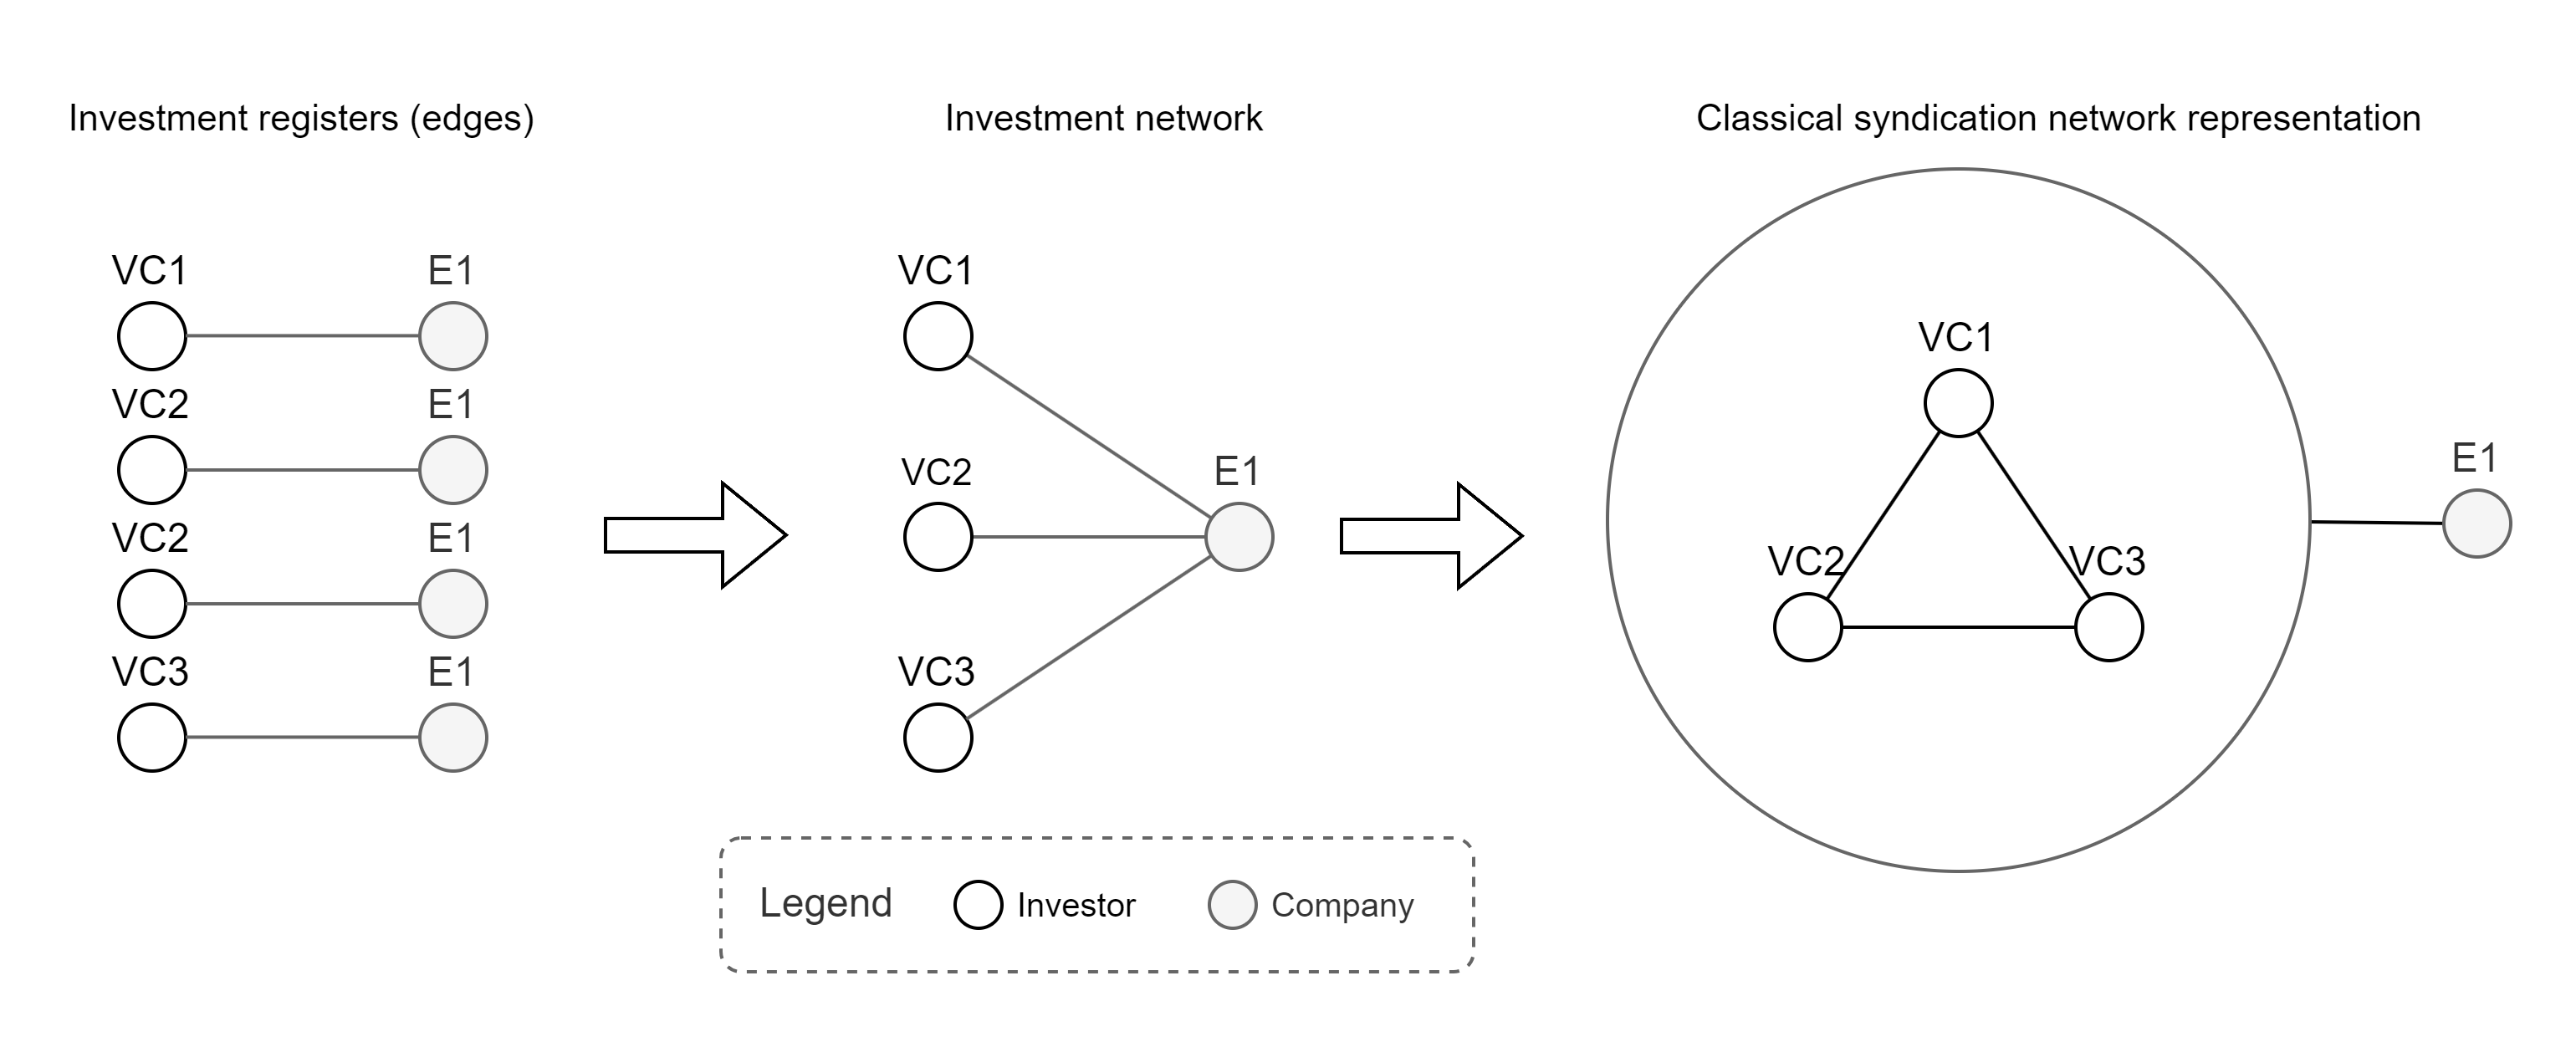
\includegraphics[width=1\textwidth]{../diagrams/classical_syndication_net.png}
    \caption{Classical syndication network: investors are connected whenever they co-invest in the same funding round. This unipartite view aggregates all investors into a single set, obscuring role differentiation and hierarchical patterns that may be present in the underlying bipartite structure.}
    \label{fig:classical_syndication_net}
\end{figure}

\subsubsection{Bipartite Projections and the Early-Late Syndication Model}

The classical syndication model described above treats all investors the same way, but in reality, investors play different roles depending on when they invest in a company's lifecycle. Our approach (detailed in our methodology) recognizes this by separating investors into two groups: early-stage investors (who fund seed and Series A rounds) and late-stage investors (who fund Series B and beyond).

This creates an early-late stage syndication model represented as a bipartite network where early-stage investors on one side connect to late-stage investors on the other side whenever they have both invested in the same company. 

The connection between our bipartite model and the classical approach lies in network projections. A projection transforms a bipartite network back into a unipartite network by connecting nodes from the same side when they share connections to the other side, as illustrated in Figure~\ref{fig:bipartite_projections}.

Mathematically, we represent our bipartite network with a biadjacency matrix $\mathbf{B}$, where $B_{uv}=1$ if early-stage investor $u$ is connected to late-stage investor $v$. The projection onto the early-stage investors is:

$$\mathbf{W}^{Early}=\mathbf{B}\mathbf{B}^{\top}$$

where $W^{Early}_{ij}$ counts how many late-stage partners two early-stage investors share. Similarly, the projection onto late-stage investors is $\mathbf{W}^{Late}=\mathbf{B}^{\top}\mathbf{B}$.

This projection mechanism provides a bridge between our role-aware bipartite model and classical syndication networks. When we project our Early-Late model, we recover something similar to classical investor-investor networks, but with the advantage of preserving distinct investor roles. This bipartite approach enables the study of hierarchical patterns like nestedness—something obscured in classical models—while ensuring compatibility with existing venture capital research.

\begin{figure}[htbp]
    \centering
    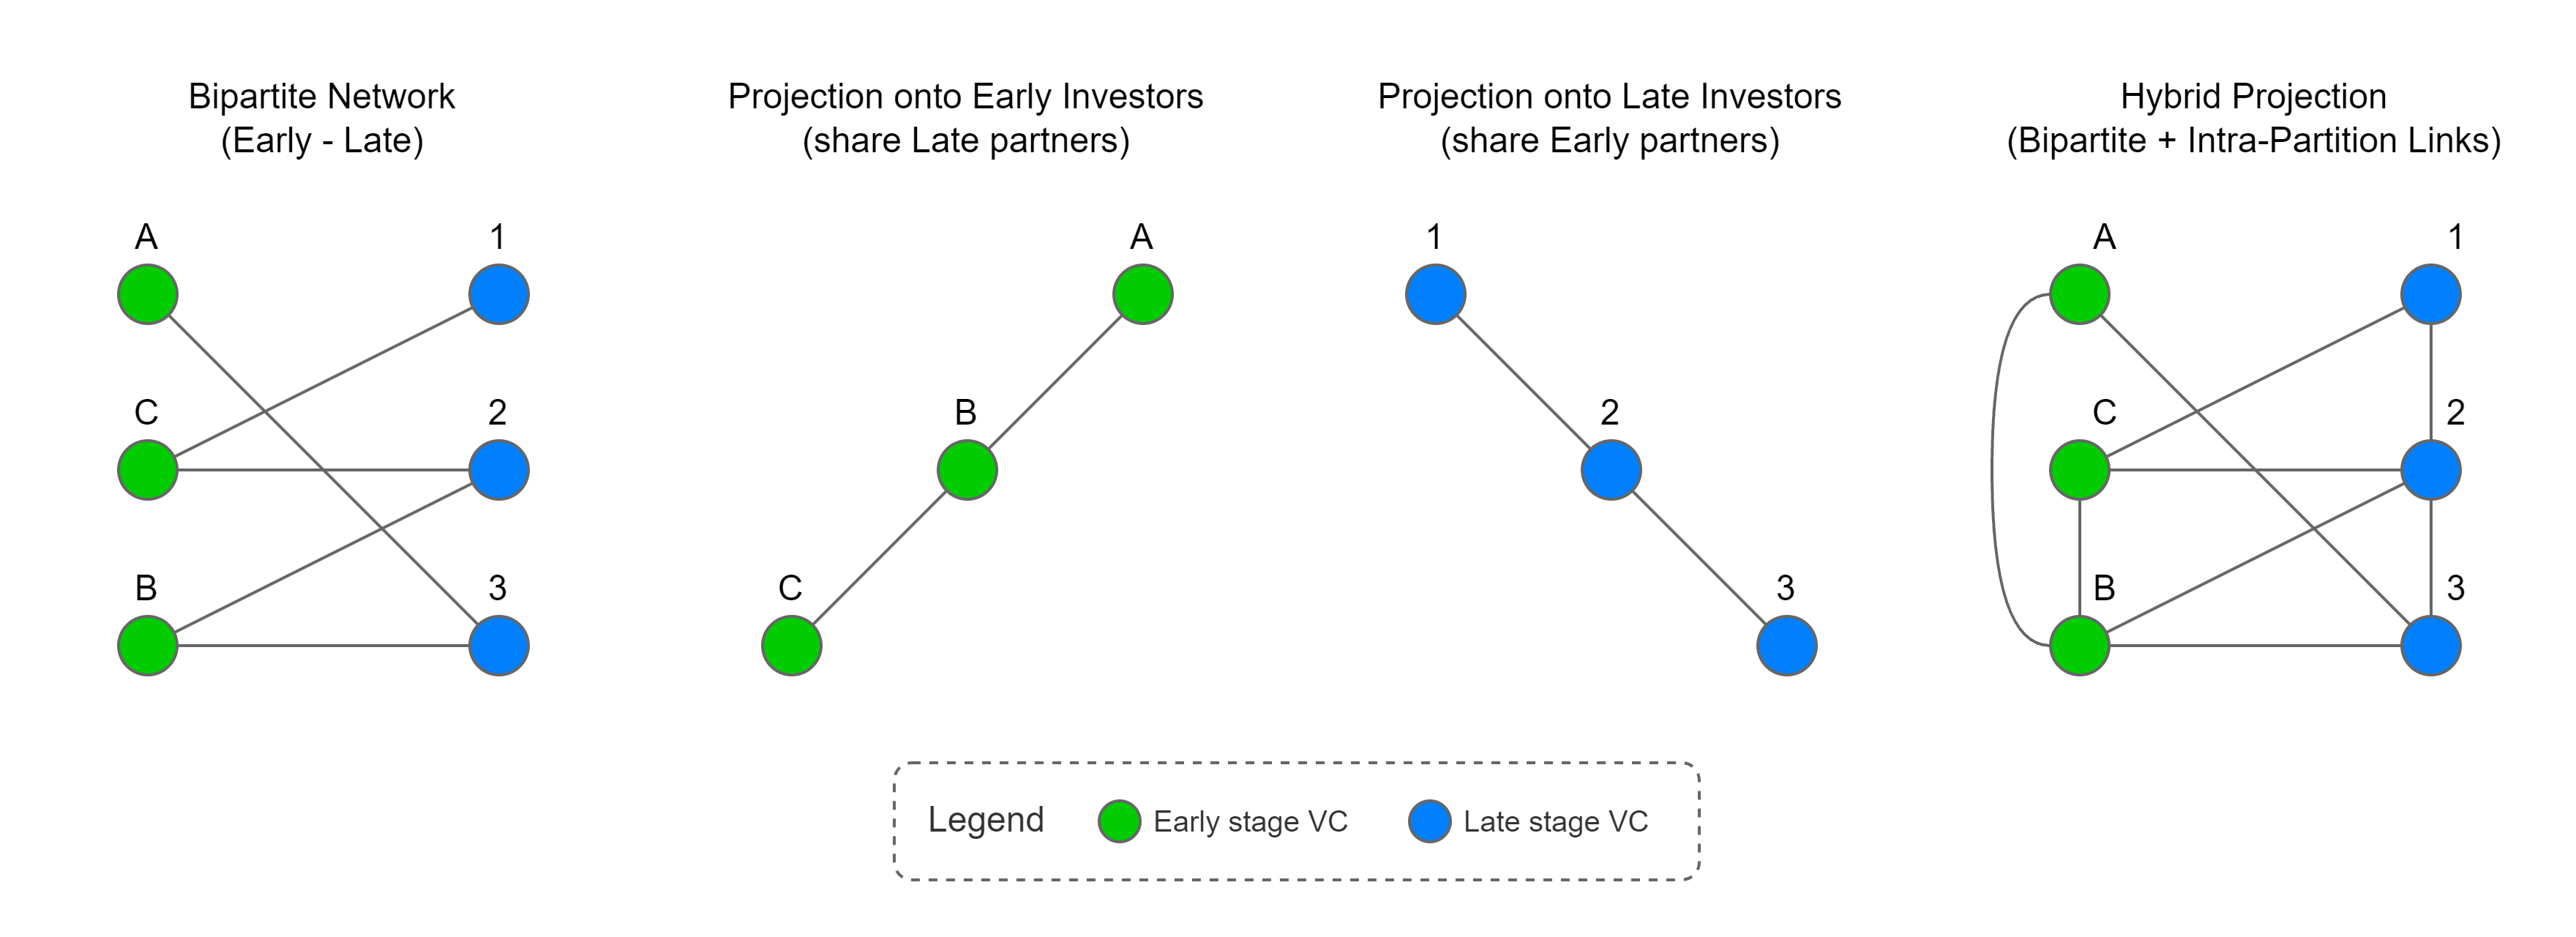
\includegraphics[width=1\textwidth]{../diagrams/bipartite_projections.png}
    \caption{Illustration of bipartite network projections. The left panel shows a bipartite graph with two disjoint node sets (e.g., Early and Late investors). The middle and right panels show the corresponding one-mode projections onto each set, where edges represent shared partners in the opposite set. This process preserves role information in the bipartite base while enabling standard network analyses in the projected graphs.}
    \label{fig:bipartite_projections}
\end{figure}

\subsubsection{Centrality, Community Structure, and Degree Patterns}

Three network concepts are particularly relevant for understanding venture capital ecosystems. First, network position and centrality metrics often quantify an investor's importance within the overall system. Highly central investors often function as gatekeepers who control information flow and access to investment opportunities \cite{Borgatti2011}. 

In fact, different centrality measures capture distinct aspects of influence: degree centrality identifies investors with many direct partnerships, while betweenness centrality identifies those who bridge otherwise disconnected investor groups.

Second, community structure reveals how investors cluster into distinct groups with denser internal connections than external ones \cite{Theophile2024}. These communities often reflect shared investment philosophies, geographic proximity, or sector specialization. 

We detect communities by maximizing \emph{modularity}, which scores a partition by comparing the observed number of within-group edges to what a degree-preserving random network would produce. In its common form,

\[
Q=\frac{1}{2m}\sum_{i,j}\left(A_{ij}-\frac{k_i k_j}{2m}\right)\delta(c_i,c_j),
\]

where $A_{ij}$ is the adjacency matrix, $k_i$ is node degree, $m$ is the number of edges, and $\delta(c_i,c_j)=1$ if $i$ and $j$ are in the same community. Louvain and Leiden algorithms search for partitions with high $Q$ \cite{Blondel2008,Traag2019}. This links naturally to the rest of our analysis: central and bridging investors can shape community boundaries, and modularity helps summarize heterogeneous, heavy-tailed connectivity into coherent groups for further study.

Last but not least, power-law degree distributions characterize the heterogeneous heavy-tailed connectivity patterns in venture capital networks \cite{Bygrave1987}. This property describes systems where a small number of investors (hubs) maintain extensive partnership networks while most participants have relatively few connections. 

Power-law distributions arise from preferential attachment mechanisms, where well-connected investors attract disproportionately more new partnerships, reflecting reputation accumulation and resource concentration dynamics.

Many real-world networks, including VC ecosystems, exhibit heavy-tailed degree distributions generated by preferential attachment dynamics \cite{Barabasi1999}, and they display small-world characteristics, combining local clustering with short global path lengths \cite{Watts1998}. 

Further, empirical evidence shows that venture capital networks consistently exhibit these power-law properties \cite{Dalle2025}, where hub investors facilitate deal flow and information diffusion throughout the ecosystem, while also creating potential bottlenecks that may limit access for entrepreneurs outside established networks. 

This structural feature creates conditions for the emergence of hierarchical organization patterns measured through, for instance, nestedness analysis.

The methodology section builds directly on these foundations by implementing community detection algorithms that identify investor clusters, while the results section examines how community structure relates to geographic distribution, investment patterns, and hierarchical organization.

\subsection{Ecology and Pollinator-Plant Networks}

The power-law degree distributions discussed above provide important insights into network structure, but they cannot fully capture the hierarchical organization patterns that emerge within investor communities.

Ecology theory offers additional insight into these organisation of complex networks. In special, studies of mutualistic pollinator-plant networks have shown that interactions often form nested structures in which specialist pollinators (those that visit few plant species) typically interact with subsets of the same plants that generalist pollinators (those that visit many species) choose \cite{Bascompte2003,Mariani2019}. 

\subsubsection{Understanding Nestedness}

To make the notion of nestedness concrete, consider a simple pollinator–plant system. Plants and pollinators form a bipartite graph where generalist species interact with many partners and specialists interact only with subsets of those partners.  

When the rows and columns of the corresponding adjacency matrix are ordered by decreasing degree, the non‑zero entries occupy the upper‑left corner, producing a characteristic triangular pattern.  

Figure~\ref{fig:nestedness_example} contrasts this bipartite representation with a standard unipartite network in which all nodes belong to the same set. The pollinator–plant analogy highlights why bipartite representations are essential for identifying hierarchical relationships like nestedness that would be obscured in one‑mode projections (unipartite networks).

\begin{figure}[htbp]
    \centering
    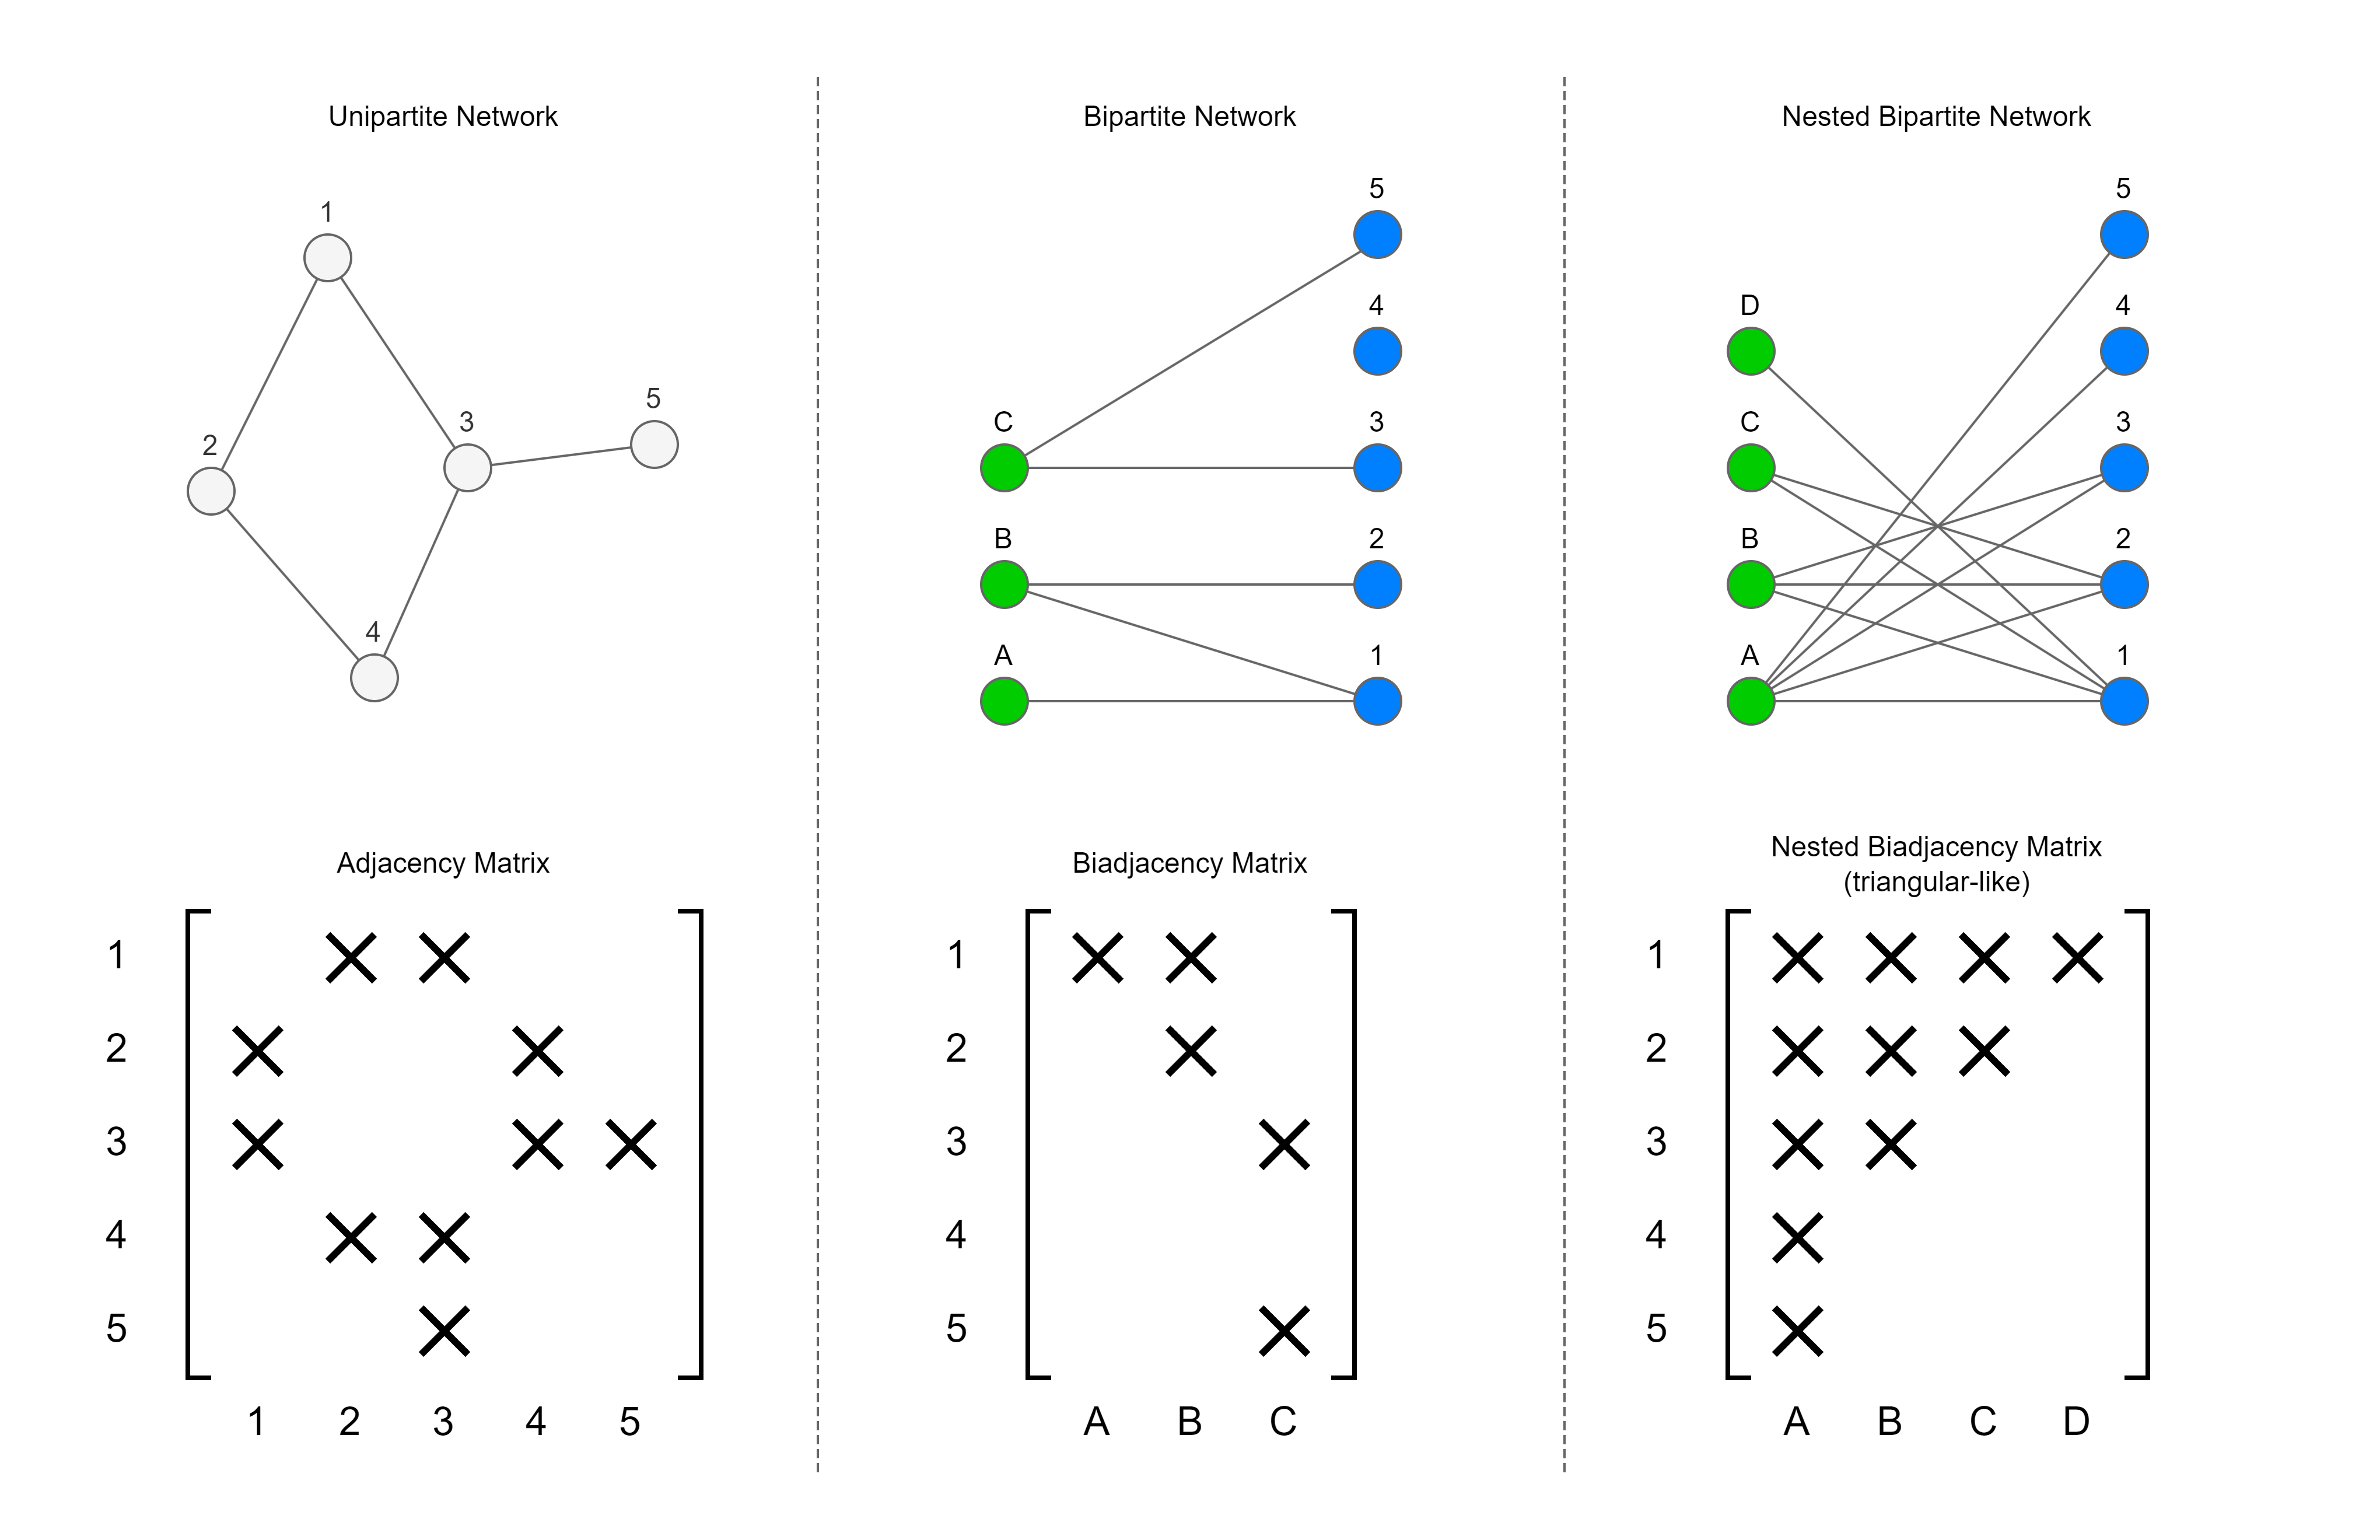
\includegraphics[width=1\textwidth]{../diagrams/unipartite_bipartite_nested_net.png}
    \caption{Illustration of nestedness in a bipartite pollinator–plant network.  Panels show, from left to right, an ordinary unipartite network, a bipartite network and a nested bipartite network together with their matrix representations.  Specialists connect to subsets of generalists’ partners, producing the triangular pattern in the bipartite matrix.}
    \label{fig:nestedness_example}
\end{figure}

Quantifying nestedness in bipartite networks has been formalised through the NODF metric \cite{AlmeidaNeto2008} and related statistical tests \cite{Ulrich2007,Dormann2009}. Nested structures can enhance robustness by allowing specialists to persist through their links to generalists, but they also concentrate influence in hubs and can increase vulnerability to targeted attacks \cite{Thebault2010,Scheffer2009}.  Recent work has explored nestedness in socio‑economic systems \cite{Mariani2019}, but its relevance for venture‑capital networks remains largely unexplored.

% Several social and economic implications are discussed around this finding, as literature defends that nested structures influence funding accessibility and overall vunerability in the entrepreneurial ecosystems. In ecology, such aspects are analog to the propensity to biodiversity (lower entry barriers) and the dilema of "stability against random species extinction" (small players) versus "vulnerability to targeted removal of highly connected species" (hubs).

% Nestedness originates from ecological studies of mutualistic relationships, particularly pollinator-plant networks. In these systems, specialist pollinators (those that visit few plant species) typically interact with subsets of the same plants that generalist pollinators (those that visit many species) choose \cite{Mariani2019}. This creates a nested hierarchy where specialists operate within the interaction networks established by generalists, rather than forming separate, independent partnerships.

% Nestedness describes this specific structural pattern where specialist nodes (those with few connections) tend to connect to subsets of the partners associated with generalist nodes (those with many connections) \cite{Mariani2019}. 

\subsubsection{Socio‑Economic Implications of Nestedness}

In socio‑economic systems, several social and economic implications are associated with nestedness, as literature defends that nested structures influence competition and overall vunerability in the  ecosystems. In ecology, such aspects are analog to the propensity to biodiversity (lower entry barriers) and the dilema of "stability against random species extinction" (small players) versus "vulnerability to targeted removal of highly connected species" (hubs).

Transposing to venture capital networks, nested behavior would mean that investors with fewer partnerships typically co-invest with a subset of the same companies that highly connected investors choose. This creates hierarchical organization where less connected investors operate within the partnership networks established by more connected ones.

This hierarchical arrangement has important implications for information flow and market access. In nested networks, information and opportunities tend to flow from generalist nodes (highly connected investors) to specialist nodes (less connected investors), creating asymmetric relationships that can influence deal flow, startup access to capital, and overall market efficiency \cite{Mariani2019}.

Nestedness patterns are particularly relevant for understanding venture capital ecosystems because they can reveal whether certain investors function as gatekeepers who control access to broader investment networks \cite{Borgatti2011}. This has direct implications for startup fundraising success and the overall efficiency of capital allocation within innovation ecosystems \cite{Theophile2024}.

% Measuring nestedness requires specialized metrics that can quantify the extent to which observed network patterns deviate from random organization. The NODF (Nestedness based on Overlap and Decreasing Fill) metric provides a standardized approach for measuring these hierarchical patterns and testing their statistical significance against null models of random network formation \cite{Mariani2019}. This methodological approach enables systematic investigation of whether investor communities exhibit meaningful hierarchical organization or operate through random partnership patterns.

\subsection{Research Questions and Contributions}

Existing VC research has shown that syndication improves deal selection and venture performance \cite{Brander2002,Sorensen2007}, yet the network‑level organisation of investor communities and its implications for financing remain unclear \cite{Pruthi2005, Benzouai2021}.  In particular, it is not known whether co‑investment networks exhibit hierarchical nestedness akin to ecological systems, how such structures relate to geographic clustering, and when they arise during the evolution of the ecosystem.

To guide the analysis, the following research questions are posed:

\begin{enumerate}
    \item Do venture‑capital syndication networks in the United States exhibit hierarchical nested structures similar to those observed in ecological mutualistic networks?
    \item How does geographic clustering, especially in Silicon Valley, influence the emergence and characteristics of nested structures in investor communities?
    \item What are the temporal dynamics of nestedness in co‑investment networks?  Do hierarchical structures emerge gradually or through phase transitions as the network grows and becomes denser?
\end{enumerate}

By answering these questions, the thesis seeks to illuminate how network topology shapes innovation financing and to provide a foundation for policy interventions aimed at fostering inclusive and resilient investment ecosystems.

The empirical analysis reveals three key contributions to the literature: First, we demonstrate significant heterogeneity in organizational structures across investor communities on US, with some exhibiting pronounced hierarchical patterns while others maintain more distributed partnership networks. Second, we identify a strong relationship between geographic clustering (particularly within Silicon Valley) and the emergence of nested organizational structures that confer measurable advantages in transaction efficiency and capital deployment. Third, we provide quantitative evidence that network topology, rather than community size alone, serves as a critical determinant of investment ecosystem performance.

The remainder of this paper presents our methodological framework, empirical findings, and their implications for understanding venture capital market organization. The Methodology section details our data preprocessing, network construction, and analytical techniques. The Results section provides comprehensive characterization of investor communities, including their geographic distributions, funding patterns, sectoral focus, and quantitative nestedness measurements. Together, these analyses offer new insights into how network structure shapes innovation financing efficiency and market access patterns.

\pagebreak